%%%%%%%%%%%%%%%%%%%%%%%%%%%%%%%%%%%%%%%%%
% Beamer Presentation
% LaTeX Template
% Version 1.0 (10/11/12)
%
% This template has been downloaded from:
% http://www.LaTeXTemplates.com
%
% License:
% CC BY-NC-SA 3.0 (http://creativecommons.org/licenses/by-nc-sa/3.0/)
%
%%%%%%%%%%%%%%%%%%%%%%%%%%%%%%%%%%%%%%%%%

%----------------------------------------------------------------------------------------
%PACKAGES AND THEMES
%----------------------------------------------------------------------------------------

\documentclass{beamer}

\mode<presentation> {

\usetheme{CambridgeUS}

\usecolortheme{dolphin}
}

\usepackage{graphicx} % Allows including images
\usepackage{booktabs} % Allows the use of \toprule, \midrule and \bottomrule in tables
\usepackage{ragged2e}
\usepackage{colortbl}

\definecolor{aliceblue}{rgb}{0.94, 0.97, 1.0} 
\definecolor{airforceblue}{rgb}{0.36, 0.54, 0.66}

%----------------------------------------------------------------------------------------
%TITLE PAGE
%----------------------------------------------------------------------------------------

\title[Streaming Data Denoising]{An Empirical Evaluation of Denoising\\Techniques for Streaming Data} % The short title appears at the bottom of every slide, the full title is only on the title page

\author{Jeremy L Thompson} % Your name
\institute[USAFA/LLNL] % Your institution as it will appear on the bottom of every slide, may be shorthand to save space
{
United States Air Force Academy\\
Lawrence Livermore National Laboratory\\ % Your institution for the title page
\medskip
\textit{jeremy.thompson@usafa.edu} % Your email address
}
\date{\today} % Date, can be changed to a custom date

\begin{document}

\begin{frame}
\titlepage % Print the title page as the first slide
\end{frame}

%------------------------------------------------

\begin{frame}
\begin{center}
\frametitle{Overview}

\justifying

We focus on denoising techniques for streaming data that is analyzed while being collected. We investigate spatial filters, such as the Box filter, Gaussian smoothing, and the Bilateral filter, and a statistical neighborhood filter, Non-Local Means.\\

$ $\\

We discuss practical concerns for incremental implementation, such as edge treatment, incremental updating, and parameter stability.\\

$ $\\

We make recommendations, specifically for the use of the Bilateral filter or a combination of the Bilateral and Non-Local Means filters.

\end{center}
\end{frame}
 
%------------------------------------------------

\begin{frame}
\frametitle{Overview} % Table of contents slide, comment this block out to remove it
\tableofcontents % Throughout your presentation, if you choose to use \section{} and \subsection{} commands, these will automatically be printed on this slide as an overview of your presentation
\end{frame}

%----------------------------------------------------------------------------------------
%PRESENTATION SLIDES
%----------------------------------------------------------------------------------------

%------------------------------------------------
\section{Background}
%------------------------------------------------

\begin{frame}
\frametitle{Noise in Real World Time Series}

\begin{columns}

\column{1.5 in}

Time Series: 

\begin{itemize}

\item Weather data

\item Test telemetry

\item Sample averages

\end{itemize}

$ $\\

Noise Sources:\\

\begin{itemize}

\item Measurement errors

\item Processing errors

\item Standard errors of the mean

\end{itemize}

\column{3 in}

\centering

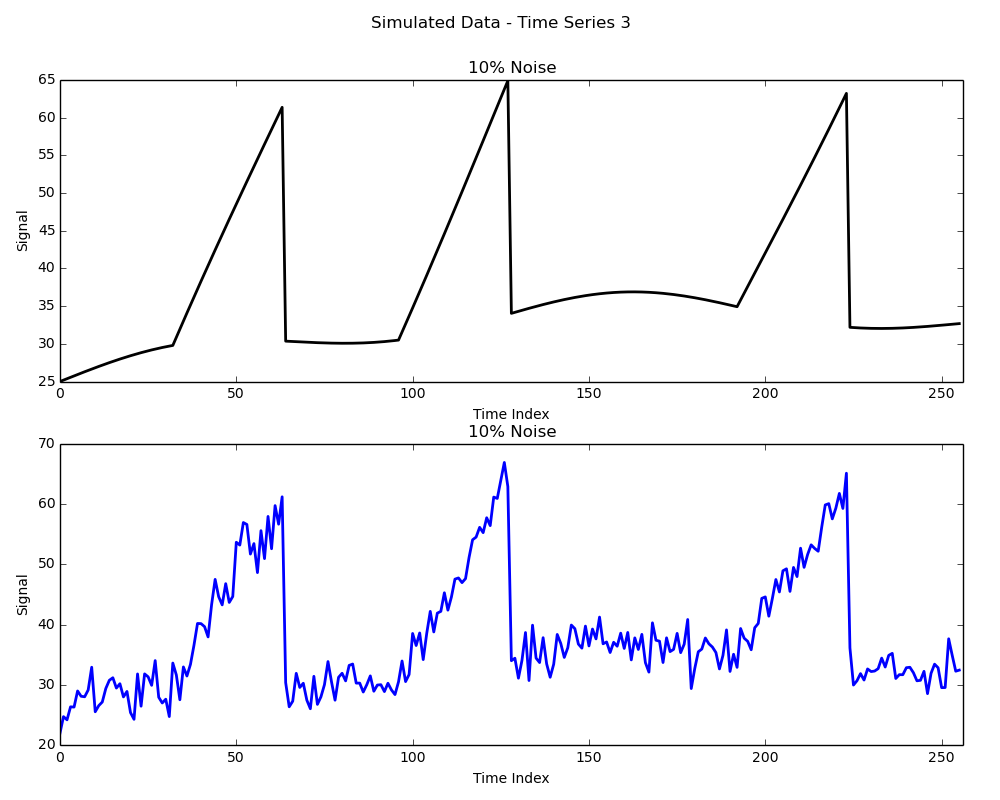
\includegraphics[width = 0.95 \textwidth]{Signal310per.png}

\end{columns}

\end{frame}

%------------------------------------------------
\section{Overview of Techniques}
%------------------------------------------------

\begin{frame}
\begin{center}
\frametitle{Notation}

Time Series - temporally orders series of observations\\

$ $\\

$y_i$ - Time series value at time index $i$\\

$s_i$ - Denoised series value at time index $i$\\

$ $\\

$ $\\

Additive White Gaussian Noise (AWGN) - error added to true time series, independent identically distributed real values from Gaussian distribution\\

$ $\\

$\sigma_n$ - standard deviation of AGWN\\

$\hat{\sigma}_n$ - estimate of $\sigma_n$

\end{center}
\end{frame}

%------------------------------------------------

\begin{frame}
\begin{center}
\frametitle{Box Filter}

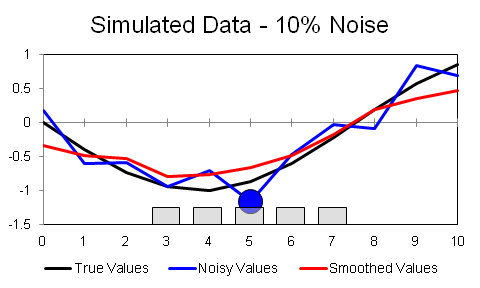
\includegraphics[width = 0.65 \textwidth]{BoxDemo.png}

\begin{columns}[c]

\column{2.5 in}
\centering

\begin{displaymath}
s_i = \sum _{j \in I} \frac{1}{\lvert I \rvert} y_j
\end{displaymath}

$ $\\

\column{2.5 in}
\justifying

Parameter:

\begin{itemize}

\item $\lvert I \rvert$ (Window Size)\\

\end{itemize}

Complexity: Low - $O \left( n \cdot \left( \frac{\lvert I \rvert - 1}{2} \right) ^2 \right)$

\end{columns}

\end{center}
\end{frame}

%------------------------------------------------

\begin{frame}
\begin{center}
\frametitle{Box Filter}

\begin{columns}

\column{0.77 \linewidth}

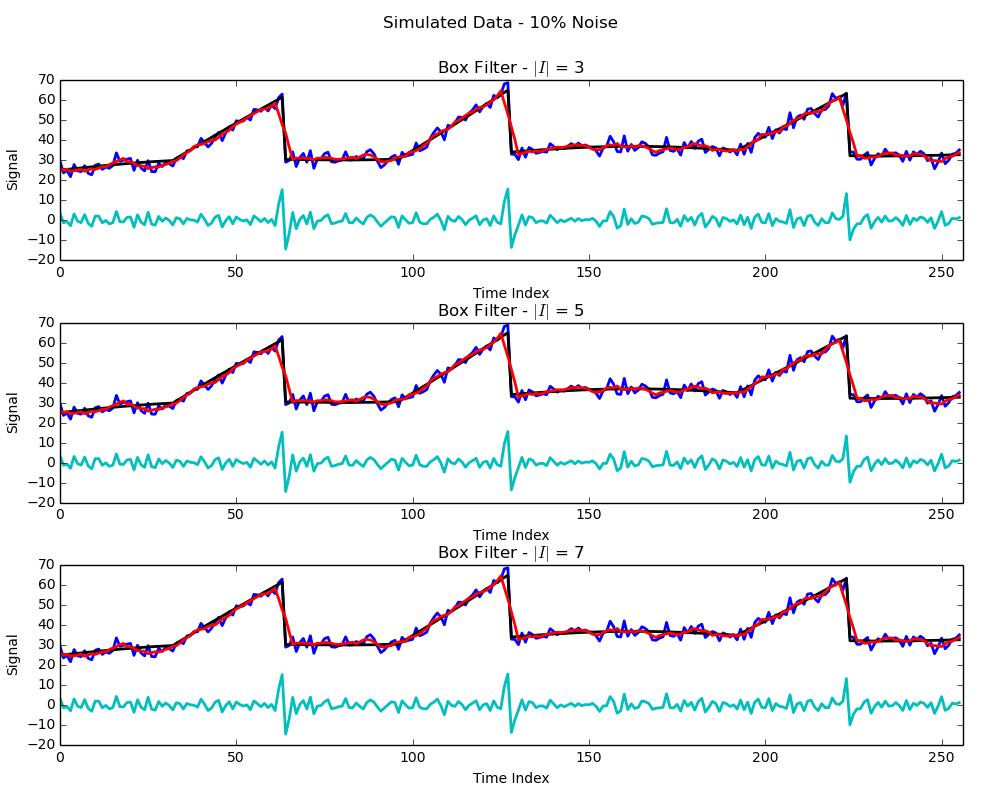
\includegraphics[width = 1.0 \textwidth]{BoxCompare.png}

\column{0.2 \linewidth}

\justifying

$\lvert I \rvert = 3$\\

$ $\\

$ $\\

$ $\\

$ $\\

$\lvert I \rvert = 5$\\

$ $\\

$ $\\

$ $\\

$ $\\

$\lvert I \rvert = 7$

\end{columns}

\end{center}
\end{frame}

%------------------------------------------------

\begin{frame}
\begin{center}
\frametitle{Gaussian Filter}

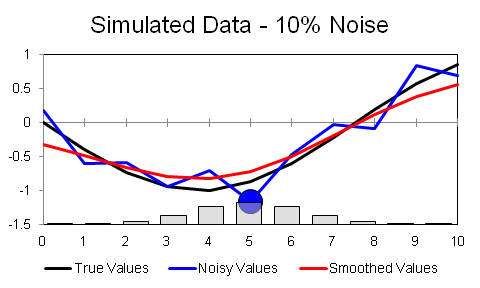
\includegraphics[width = 0.65 \textwidth]{GaussianDemo.png}

\begin{columns}[c]

\column{2.5 in}
\centering

\begin{displaymath}
s_i = \sum _{j \in I} \frac{1}{z_i} e^{-\frac{\lvert i - j \rvert}{2 \sigma_d^2}} y_j
\end{displaymath}

$ $\\

\column{2.5 in}
\justifying

Parameter:

\begin{itemize}

\item $\sigma_d$ (Spatial Kernel)

\end{itemize}

Complexity: Low - $O \left( n \cdot \lfloor 5 \sigma_d \rfloor ^2 \right)$

\end{columns}

\end{center}
\end{frame}

%------------------------------------------------

\begin{frame}
\begin{center}
\frametitle{Gaussian Filter}

\begin{columns}

\column{0.77 \linewidth}

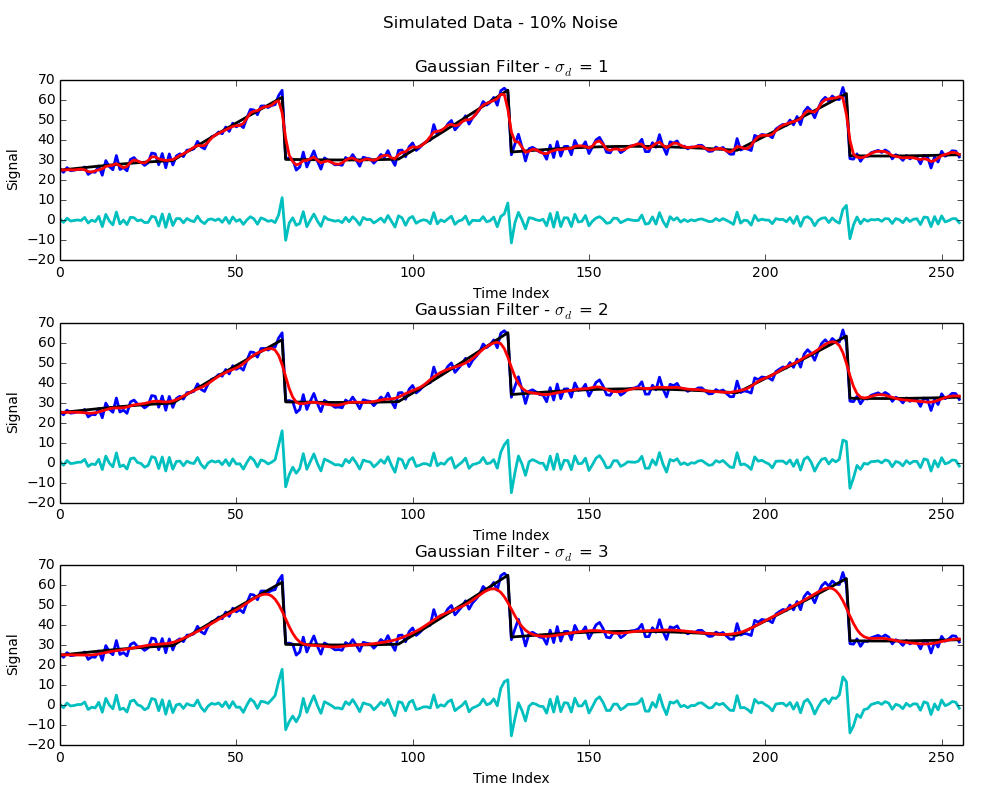
\includegraphics[width = 1.0 \textwidth]{GaussianCompare.png}

\column{0.2 \linewidth}

\justifying

$\sigma_d = 1.0$\\

$ $\\

$ $\\

$ $\\

$ $\\

$\sigma_d = 2.0$\\

$ $\\

$ $\\

$ $\\

$ $\\

$\sigma_d = 3.0$

\end{columns}

\end{center}
\end{frame}

%------------------------------------------------

\begin{frame}
\begin{center}
\frametitle{Bilateral Filter}

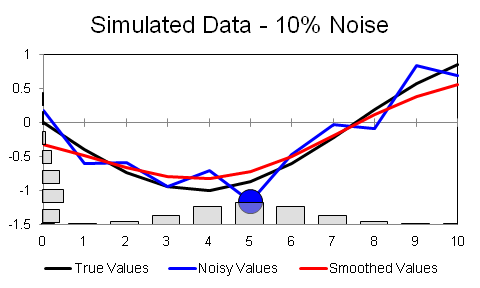
\includegraphics[width = 0.65 \textwidth]{BilateralDemo.png}

\begin{columns}[c]

\column{2.25 in}
\centering

\begin{displaymath}
s_i = \sum _{j \in I} \frac{1}{z_i} e^{-\frac{\lvert i - j \rvert}{2 \sigma_d^2}}e^{-\frac{\lvert y_i - y_j \rvert}{2 \sigma_i^2}} y_j
\end{displaymath}

$ $\\

\column{3.25 in}
\justifying

Parameters:

\begin{itemize}

\item $\sigma_d$ (Spatial Kernel)

\item $\sigma_i = k \hat{\sigma}_n$ (Intensity Kernel)

\end{itemize}

Complexity: Moderate - $O \left( n \cdot \log \lfloor 5 \sigma_d \rfloor \right)$\\

\end{columns}

\end{center}
\end{frame}

%------------------------------------------------

\begin{frame}
\begin{center}
\frametitle{Bilateral Filter}

\begin{columns}

\column{0.77 \linewidth}

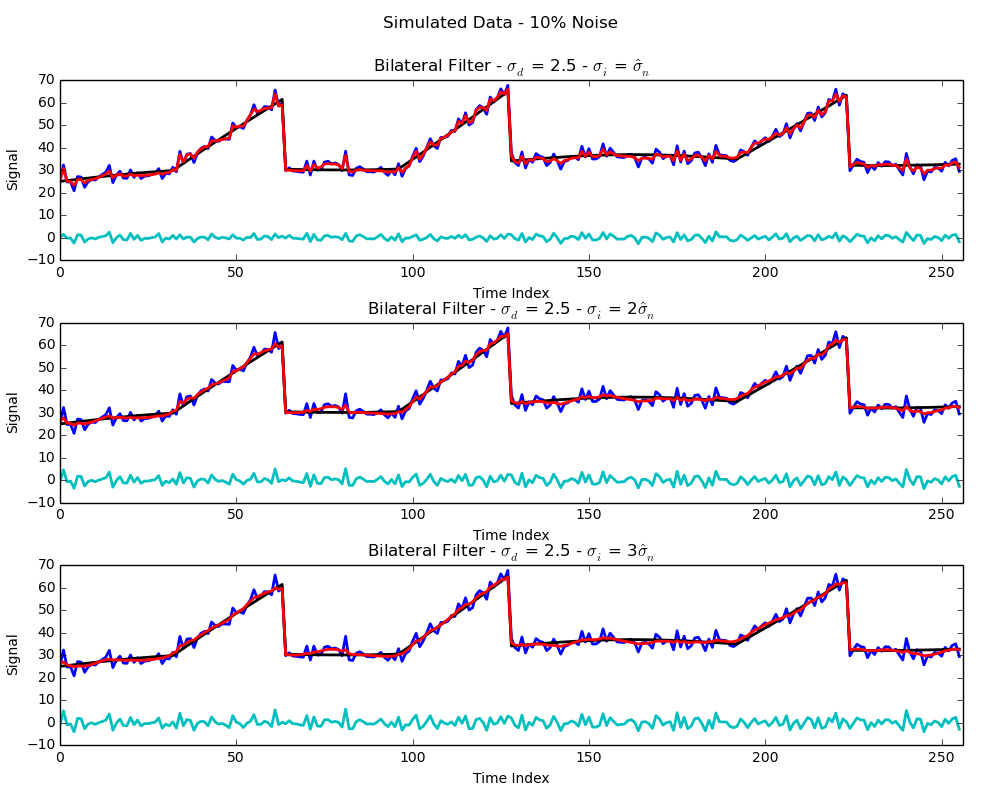
\includegraphics[width = 1.0 \textwidth]{BilateralCompare.png}

\column{0.2 \linewidth}

\justifying

$\sigma_d = 2.5$\\

$\sigma_i = 1.0 \hat{\sigma}_n$\\

$ $\\

$ $\\

$ $\\

$\sigma_d = 2.5$\\

$\sigma_i = 2.0 \hat{\sigma}_n$\\

$ $\\

$ $\\

$ $\\

$\sigma_d = 2.5$\\

$\sigma_i = 3.0 \hat{\sigma}_n$

\end{columns}

\end{center}
\end{frame}

%------------------------------------------------

\begin{frame}
\begin{center}
\frametitle{Non-Local Means Filter}

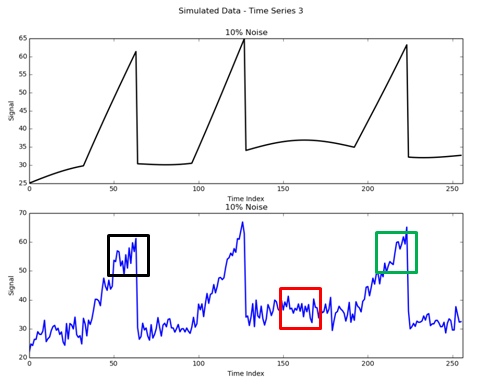
\includegraphics[width = 0.45 \textwidth]{NLMeansDemo.png}

\small{

\begin{columns}

\column{2.5 in}

\begin{displaymath}
s_i = \sum _{j \in N}
\begin{cases}
\frac{1}{z_i} e^{-\frac{\lvert Y_i - Y_j \rvert ^2}{2 \beta \hat{\sigma}^2_n \lvert I \rvert}} y_j & \lvert Y_i - Y_j \rvert < T \\
0 & $otherwise$
\end{cases}
\end{displaymath}

$Y_j$ - vector of time series values around $y_j$\\

$ $\\

$ $\\

\column{2.5 in}
\justifying

Parameters:

\tiny{

\begin{itemize}

\item $\beta$ (Smoothing Level)

\item $\lvert I \rvert$ (Window Size)

\item $T = k \left( \mathrm{max} Y_j - \mathrm{min} Y_j \right) \lvert I \rvert$ (Pre-selection Threshold)

\end{itemize}

}

\small{

Complexity: High - $O \left( n^3 \right)$

}

\end{columns}
}

\end{center}
\end{frame}

%------------------------------------------------

\begin{frame}
\begin{center}
\frametitle{Non-Local Means Filter}

\begin{columns}

\column{0.77 \linewidth}

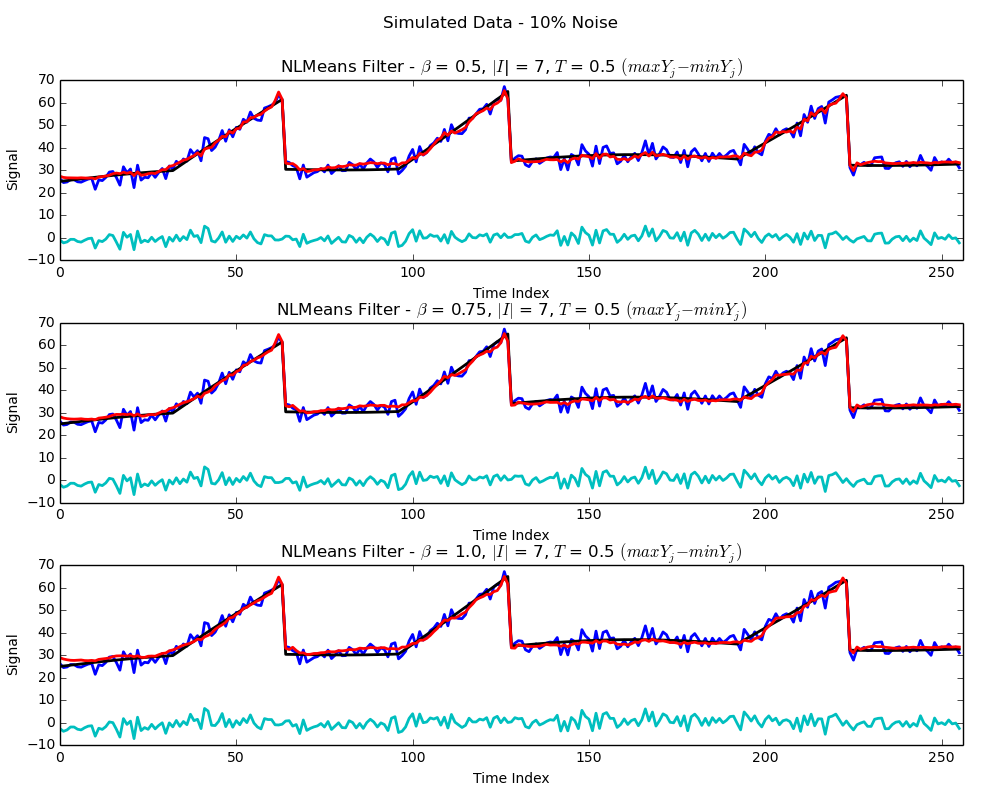
\includegraphics[width = 1.0 \textwidth]{NLMeansCompare.png}

\column{0.2 \linewidth}

\justifying

\tiny{

$\beta = 0.5$\\

$\lvert I \rvert = 7$\\

$T =$ \\ $0.5 \left( \mathrm{max} Y_j - \mathrm{min} Y_j \right) \lvert I \rvert$\\

$ $\\

$ $\\

$ $\\

$ $\\

$ $\\

$\beta = 0.75$\\

$\lvert I \rvert = 7$\\

$T =$ \\ $0.5 \left( \mathrm{max} Y_j - \mathrm{min} Y_j \right) \lvert I \rvert$\\

$ $\\

$ $\\

$ $\\

$ $\\

$ $\\

$\beta = 1.0$\\

$\lvert I \rvert = 7$\\

$T =$ \\ $0.5 \left( \mathrm{max} Y_j - \mathrm{min} Y_j \right) \lvert I \rvert$

}

\end{columns}

\end{center}
\end{frame}

%------------------------------------------------

\begin{frame}
\begin{center}
\frametitle{Frequency Techniques}

\begin{columns}[t]

\column{0.6 \linewidth}
\centering

Fourier Transform

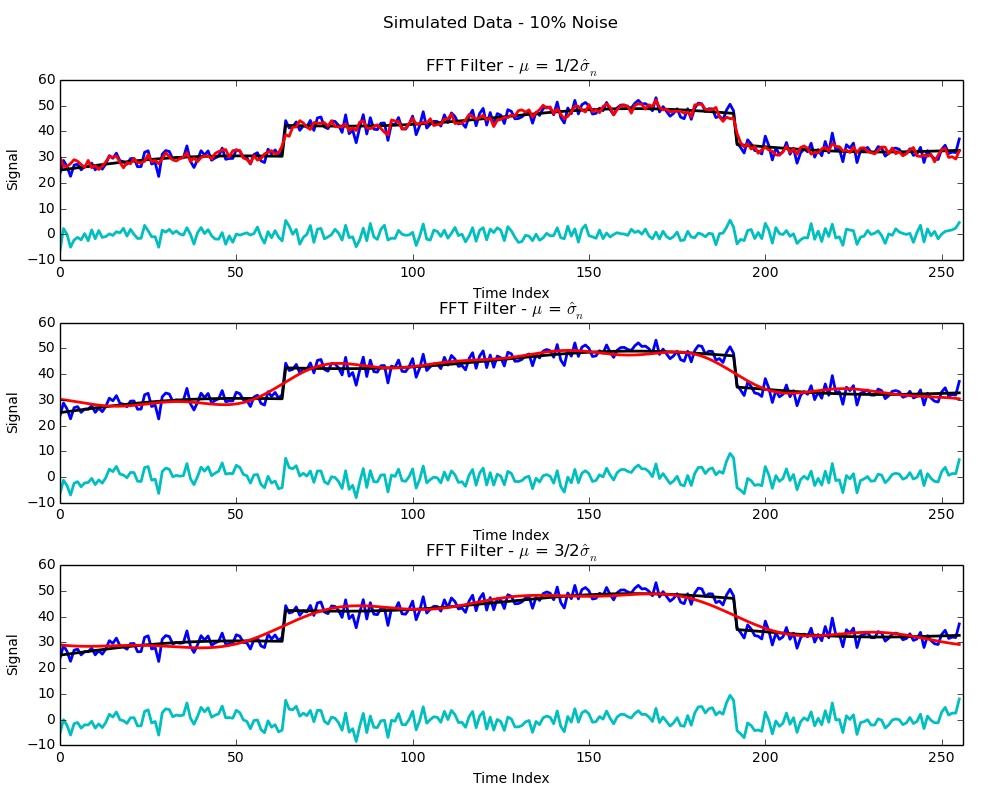
\includegraphics[width = 0.9 \textwidth]{FFTCompare.png}

\column{0.4 \linewidth}
\centering

Wavelet Transform\\

\justifying

$ $\\

Parameters/Options:

\begin{itemize}

\item Wavelet family

\item Number of levels

\item Threshold type

\item Threshold cut-off

\end{itemize}

\end{columns}

$ $\\

$ $\\

Fourier Transform and Wavelets - considered but not discussed

\end{center}
\end{frame}

%------------------------------------------------
\section{Practical Concerns}
%------------------------------------------------

\begin{frame}
\begin{center}
\frametitle{Practical Concerns}

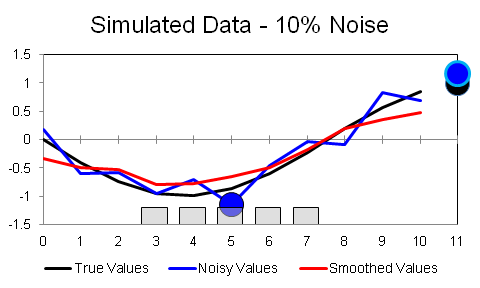
\includegraphics[width = 0.65 \textwidth]{IncrementOverview.png}

Typically denosing methods don't explicitly describe edge treatment...\\

$ $\\

but the leading edge is most relevant portion of real-time time series

\end{center}
\end{frame}

%------------------------------------------------

\begin{frame}
\begin{center}
\frametitle{Spatial Filters}

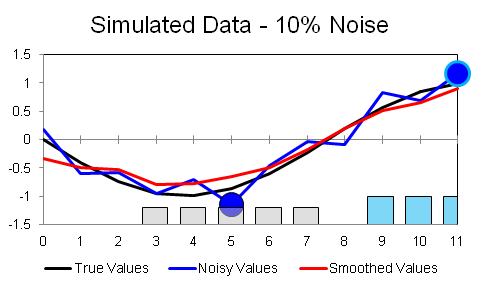
\includegraphics[width = 0.65 \textwidth]{Edge.png}

Problem: Incomplete windows to average over on edges\\

$ $\\

Solution: Average over the portion of the window that is available

\end{center}
\end{frame}

%------------------------------------------------

\begin{frame}
\begin{center}
\frametitle{Spatial Filters}

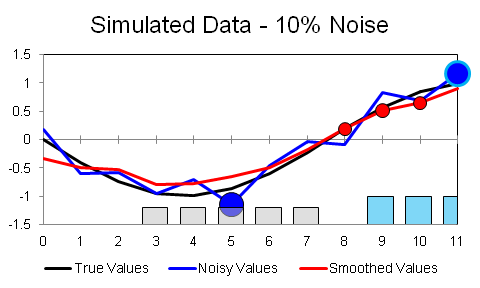
\includegraphics[width = 0.65 \textwidth]{Increment.png}

Incremental Updating: when new data is received, update only the smoothed values of the previous edge values and add new smoothed value

\end{center}
\end{frame}

%------------------------------------------------

\begin{frame}
\begin{center}
\frametitle{Non-Local Means Filter}

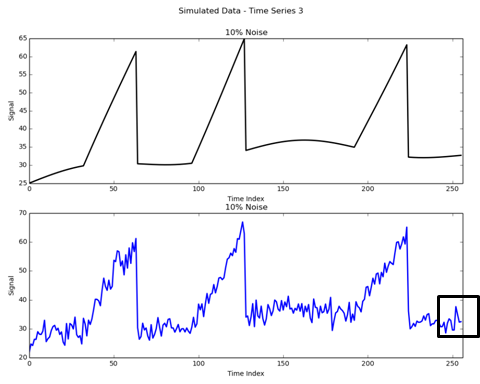
\includegraphics[width = 0.45 \textwidth]{NLMeansEdge.png}

Problem: Incomplete windows to compare on edges\\

$ $\\

Solution: Compare the portion of the window that is available

\end{center}
\end{frame}

%------------------------------------------------

\begin{frame}
\begin{center}
\frametitle{Non-Local Means Filter}

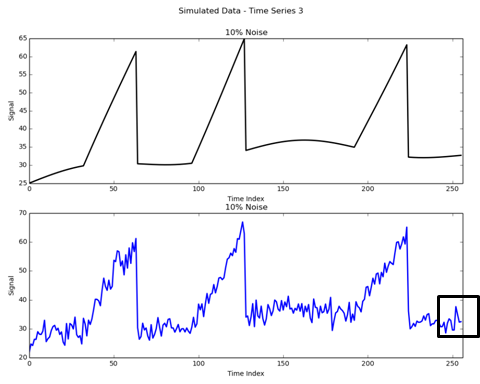
\includegraphics[width = 0.45 \textwidth]{NLMeansEdge.png}

Incremental Updating: when new data is received, update only the smoothed values of the previous edge values and add new smoothed value

\end{center}
\end{frame}

%------------------------------------------------
\section{Parameter Stability}
%------------------------------------------------

\begin{frame}
\begin{center}
\frametitle{Parameter Stability}

There are parameter optimization techniques, but

\begin{itemize}

\item Our data is dynamic

\item Optimization takes time

\item Bad parameters can destroy information

\item Difficult to know if smoothed series is 'good'

\end{itemize}

$ $\\

$ $\\

Goal: Find methods/parameters that are stable across a variety of signals\\

$ $\\

Solution: DOE/grid search for optimal PSNR on known time series

\end{center}
\end{frame}

%------------------------------------------------

\begin{frame}
\begin{center}
\frametitle{PSNR}

\begin{columns}

\column{0.65 \linewidth}

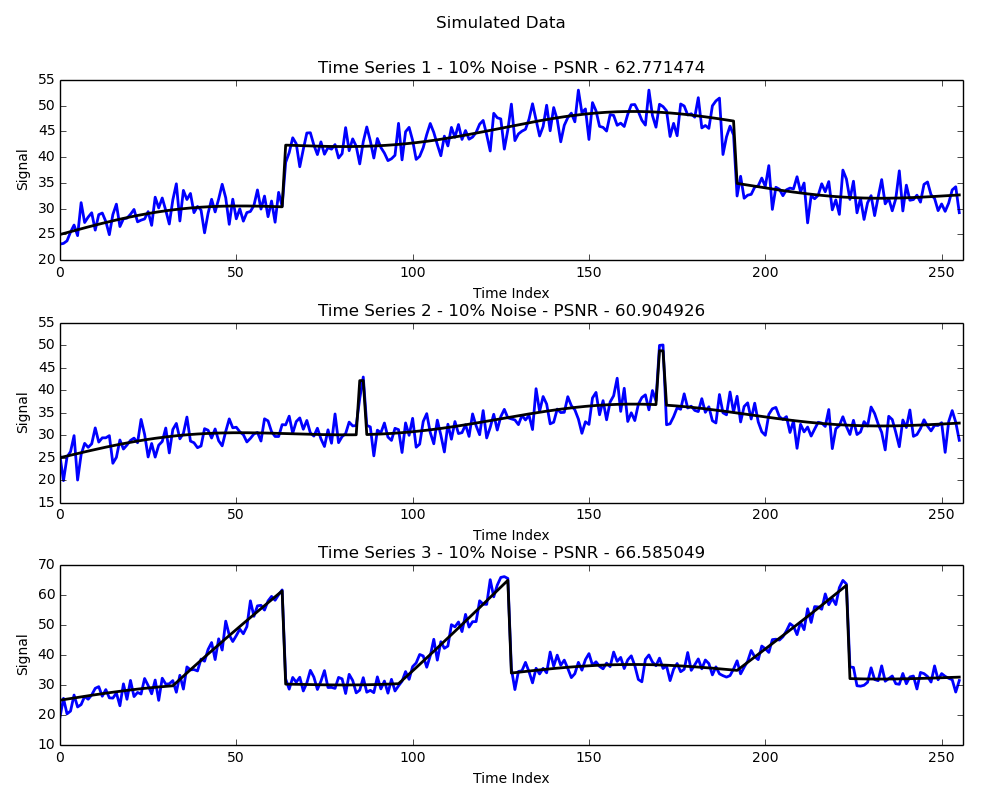
\includegraphics[width = 1.0 \textwidth]{SignalsCompare.png}

\column{0.35 \linewidth}

\centering

\small{

$ $\\

Time Series 1\\

$PSNR = 62.771$\\

$ $\\

$ $\\

$ $\\

Time Series 2\\

$PSNR = 60.905$\\

$ $\\

$ $\\

$ $\\

Time Series 3\\

$PSNR = 66.585$

$ $\\

}

\end{columns}

\small{

\begin{columns}

\column{2.5 in}

\centering

PSNR - Peak Signal to Noise Ratio\\

$PSNR = 10 log_{10} \left( \frac{\left(\mathrm{max} y_i \right) ^2}{MSE} \right)$\\

\column{2.5 in}

\centering

$MSE = \frac{1}{n} \sum _{i \in N} \left( \hat{y}_i - y_i \right) ^2$

\end{columns}

}

\end{center}
\end{frame}

%------------------------------------------------

\begin{frame}
\begin{center}
\frametitle{DOE/Grid Search}

Investigated smoothing performance at grid points and\\increased resolution in areas of interest\\

\begin{itemize}

\item Noise: $1$\%, $5$\%, $10$\%, $20$\%, and $30$\%

\item $\lvert I \rvert$: $3$, $5$, $7$, and $9$

\item $\sigma_d$: $0.1$, $1.0$, $2.0$, $3.0$, and $4.0$

\item $\sigma_i$: $0.1 \hat{\sigma}_n$, $1.0 \hat{\sigma}_n$, $2.0 \hat{\sigma}_n$, $3.0 \hat{\sigma}_n$,  and $4.0 \hat{\sigma}_n$

\item $\beta$: $0.5$, $0.75$, and $1.0$

\item $T$: $0.25 \left( \mathrm{max} Y_j - \mathrm{min} Y_j \right) \lvert I \rvert$, $0.5 \left( \mathrm{max} Y_j - \mathrm{min} Y_j \right) \lvert I \rvert$, and $0.75 \left( \mathrm{max} Y_j - \mathrm{min} Y_j \right) \lvert I \rvert$

\end{itemize}

\end{center}
\end{frame}

%------------------------------------------------

\begin{frame}
\begin{center}
\frametitle{Box Filter}

\small{

PSNR - Optimal Settings

\begin{table}[h]
\begin{tabular}{l | l | l | l}
 & Time Series 1 & Time Series 2 & Time Series 3 \\ \hline
1\% Noise & 85.594 & 72.175 & 67.346 \\ \hline
5\% Noise & 81.206 & 70.377 & 66.771 \\ \hline
10\% Noise & 74.047 & 66.201 & 65.354 \\ \hline
20\% Noise & 64.323 & 58.005 & 60.920 \\ \hline
30\% Noise & 56.888 & 52.199 & 57.145
\end{tabular}
\end{table}

PSNR - $\lvert I \rvert = 7$

\begin{table}[h]
\begin{tabular}{l | l | l | l}
 & Time Series 1 & Time Series 2 & Time Series 3 \\ \hline
1\% Noise &85.549/99.9\% &72.175/100.0\% &67.346/100.0\% \\ \hline
5\% Noise &81.059/99.8\% &70.181/99.7\% & 66.747/100.0\% \\ \hline
10\% Noise &73.249/98.9\% &66.040/99.8\% & 64.923/99.3\% \\ \hline
20\% Noise &62.786/97.6\% &57.932/99.9\% &60.631/99.5\% \\ \hline
30\% Noise &56.165/98.7\% &51.829/99.3\% &56.082/98.1\%
\end{tabular}
\end{table}

}

\end{center}
\end{frame}

%------------------------------------------------

\begin{frame}
\begin{center}
\frametitle{Box Filter}

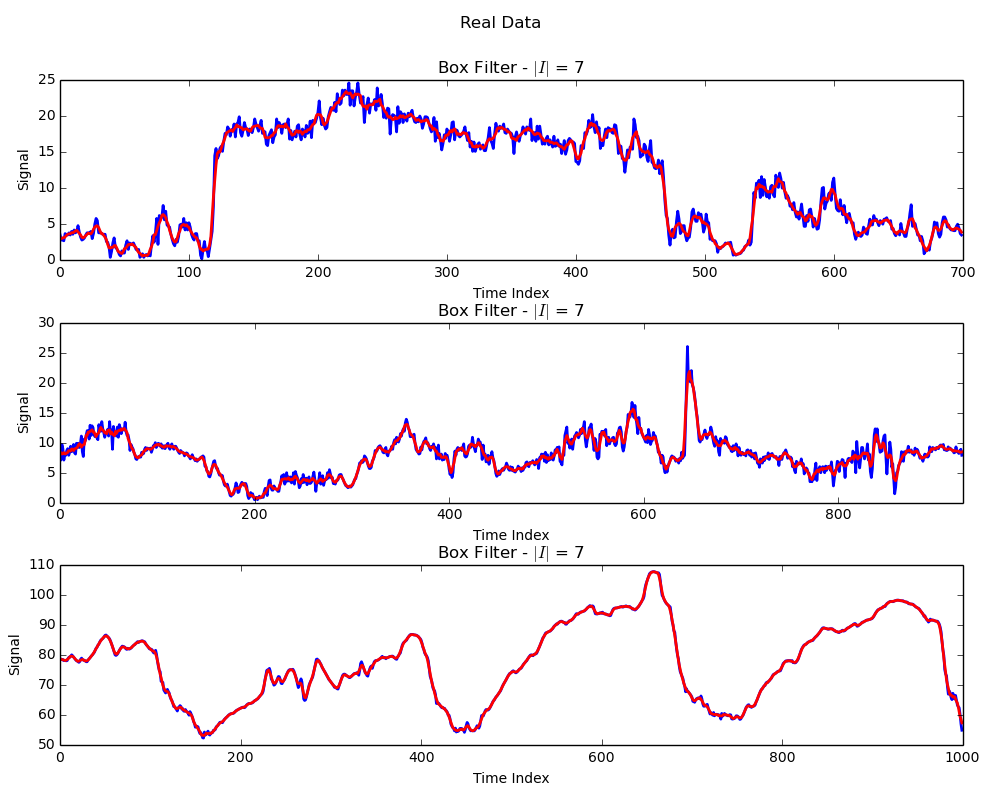
\includegraphics[width = 0.75 \textwidth]{BoxRealCompare.png}

\end{center}
\end{frame}

%------------------------------------------------

\begin{frame}
\begin{center}
\frametitle{Gaussian Filter}

\small{

PSNR - Optimal Settings

\begin{table}[h]
\begin{tabular}{l | l | l | l}
 & Time Series 1 & Time Series 2 & Time Series 3 \\ \hline
1\% Noise & 83.257 & 71.659 & 74.807 \\ \hline
5\% Noise & 80.684 & 70.459 & 79.871 \\ \hline
10\% Noise & 75.844 & 68.646 & 69.177 \\ \hline
20\% Noise & 69.529 & 60.971 & 62.031 \\ \hline
30\% Noise & 61.243 & 56.495 & 58.172
\end{tabular}
\end{table}

PSNR - $\sigma_d = 2.25$

\begin{table}[h]
\begin{tabular}{l | l | l | l}
 & Time Series 1 & Time Series 2 & Time Series 3 \\ \hline
1\% Noise & 83.257/100.0\% & 71.659/100.0\% & 63.953/85.5\% \\ \hline
5\% Noise & 80.684/100.0\% & 70.459/100.0\% & 63.685/79.7\% \\ \hline
10\% Noise & 75.844/100.0\% & 67.568/98.4\% & 62.980/91.0\% \\ \hline
20\% Noise & 67.086/96.5\% & 60.005/98.4\% & 60.437/97.4\% \\ \hline
30\% Noise & 59.973/97.9\% & 54.554/96.6\% & 56.797/97.6\%
\end{tabular}
\end{table}

}

\end{center}
\end{frame}

%------------------------------------------------

\begin{frame}
\begin{center}
\frametitle{Gaussian Filter}

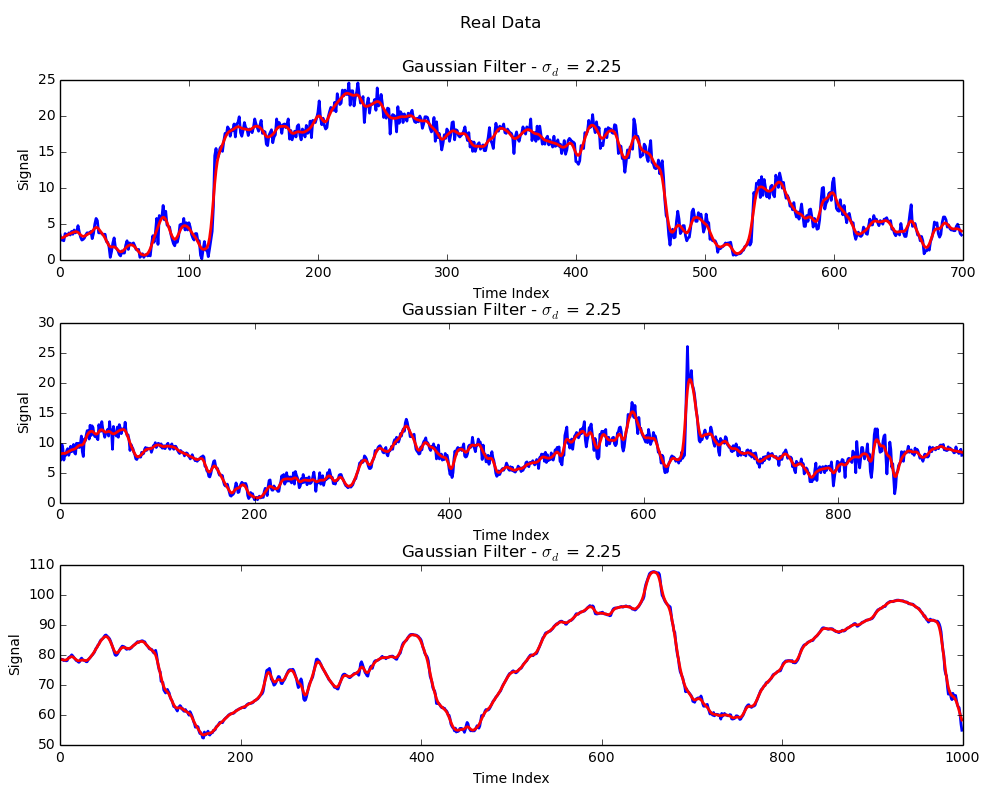
\includegraphics[width = 0.75 \textwidth]{GaussianRealCompare.png}

\end{center}
\end{frame}

%------------------------------------------------

\begin{frame}
\begin{center}
\frametitle{Bilateral Filter}

\small{

PSNR - Optimal Settings

\begin{table}[h]
\begin{tabular}{l | l | l | l}
 & Time Series 1 & Time Series 2 & Time Series 3 \\ \hline
1\% Noise & 127.251 & 128.396 & 121.790 \\ \hline
5\% Noise & 97.303 & 96.758 & 96.698 \\ \hline
10\% Noise & 81.774 & 78.128 & 84.987 \\ \hline
20\% Noise & 69.794 & 63.453 & 70.033 \\ \hline
30\% Noise & 62.657 & 59.049 & 61.736
\end{tabular}
\end{table}

PSNR - $\sigma_d = 2.5$, $\sigma_i = 2.5 \hat{\sigma}_n$

\begin{table}[h]
\begin{tabular}{l | l | l | l}
1\% Noise & 124.947/98.2\% & 126.752/98.7\% & 110.432/90.7\% \\ \hline
5\% Noise & 93.220/95.8\% & 92.841/96.0\% & 96.698/100.0\% \\ \hline
10\% Noise & 79.580/97.3\% & 75.578/96.7\% & 84.480/99.4\% \\ \hline
20\% Noise & 64.659/92.6\% & 60.585/95.5\% & 68.456/97.7\% \\ \hline
30\% Noise & 57.875/92.4\% & 53.774/91.1\% & 60.891/98.6\%
\end{tabular}
\end{table}

}

\end{center}
\end{frame}

%------------------------------------------------

\begin{frame}
\begin{center}
\frametitle{Bilateral Filter}

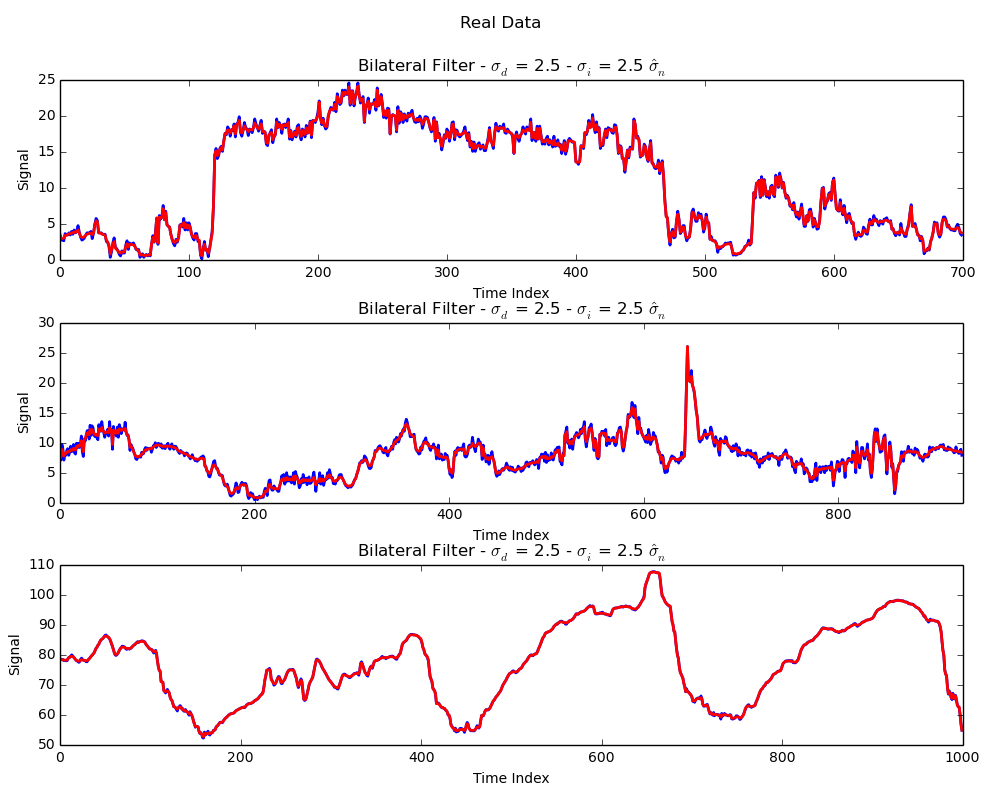
\includegraphics[width = 0.75 \textwidth]{BilateralRealCompare.png}

\end{center}
\end{frame}

%------------------------------------------------

\begin{frame}
\begin{center}
\frametitle{Non-Local Means Filter}

\small{

PSNR - Optimal Settings

\begin{table}[h]
\begin{tabular}{l | l | l | l}
 & Time Series 1 & Time Series 2 & Time Series 3 \\ \hline
1\% Noise & 114.852 & 112.238 & 101.050 \\ \hline
5\% Noise & 89.317 & 89.332 & 92.007 \\ \hline
10\% Noise & 77.760 & 75.828 & 79.996 \\ \hline
20\% Noise & 65.997 & 60.698 & 68.439 \\ \hline
30\% Noise & 58.928 & 54.630 & 62.217
\end{tabular}
\end{table}

PSNR - $\beta = 0.5$, $\lvert I \rvert = 7$, $T = 0.75 \left( \mathrm{max} Y_j - \mathrm{min} Y_j \right)$

\begin{table}[h]
\begin{tabular}{l | l | l | l}
1\% Noise & 114.852/98.0\% & 112.238/98.1\% & 101.050/98.0\% \\ \hline
5\% Noise & 89.317/98.6\% & 89.332/97.4\% & 92.007/98.1\% \\ \hline
10\% Noise & 77.760/95.7\% & 75.828/95.1\% & 79.996/98.8\% \\ \hline
20\% Noise & 65.997/95.5\% & 60.698/95.0\% & 68.439/96.6\% \\ \hline
30\% Noise & 58.928/96.5\% & 54.630/99.6\% & 62.217/96.1\%
\end{tabular}
\end{table}

}

\end{center}
\end{frame}

%------------------------------------------------

\begin{frame}
\begin{center}
\frametitle{Non-Local Means Filter}

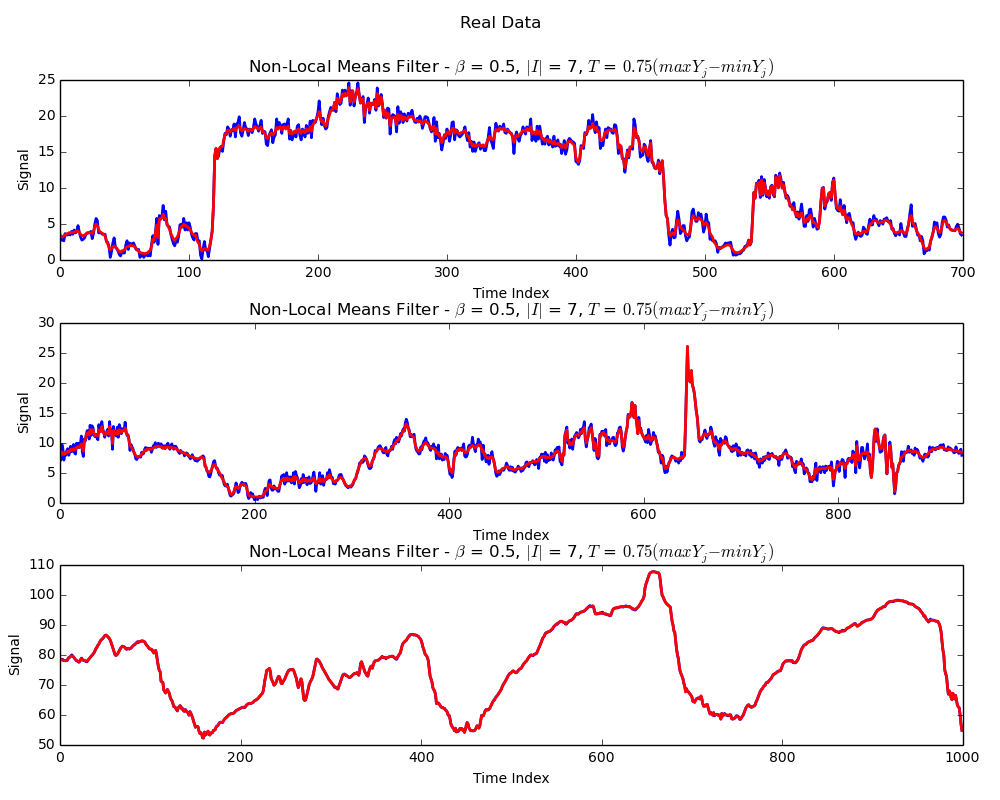
\includegraphics[width = 0.75 \textwidth]{NLMeansRealCompare.png}

\end{center}
\end{frame}

%------------------------------------------------

\begin{frame}
\begin{center}
\frametitle{Bilateral and Non-Local Means Filters Combination}

\small{

PSNR - Optimal Settings

\begin{table}[h]
\begin{tabular}{l | l | l | l}
 & Time Series 1 & Time Series 2 & Time Series 3 \\ \hline
1\% Noise & 116.272 & 114.415 & 110.231 \\ \hline
5\% Noise & 100.498 & 97.932 & 97.620 \\ \hline
10\% Noise & 87.153 & 82.641 & 86.879 \\ \hline
20\% Noise & 73.244 & 66.868 & 75.505 \\ \hline
30\% Noise & 67.219 & 60.023 & 84.472
\end{tabular}
\end{table}

PSNR - $\sigma_d = 2.5$, $\sigma_i = 1.8 \hat{\sigma}_n$, $\beta = 0.5$, $\lvert I \rvert = 7$, $T = 0.9 \left( \mathrm{max} Y_j - \mathrm{min} Y_j \right)$

\begin{table}[h]
\begin{tabular}{l | l | l | l}
1\% Noise & 114.572/98.5\% & 111.731/97.7\% & 94.137/85.4\% \\ \hline
5\% Noise & 94.730/94.3\% & 94.948/97.0\% & 89.549/91.7\% \\ \hline
10\% Noise & 79.659/91.4\% & 78.388/94.9\% & 77.953/89.7\% \\ \hline
20\% Noise & 66.427/90.7\% & 61.955/92.7\% & 66.799/88.5\% \\ \hline
30\% Noise & 60.274/89.7\% & 57.825/96.3\% & 84.472/100.0\%
\end{tabular}
\end{table}

}

\end{center}
\end{frame}

%------------------------------------------------

\begin{frame}
\begin{center}
\frametitle{Bilateral and Non-Local Means Filters Combination}

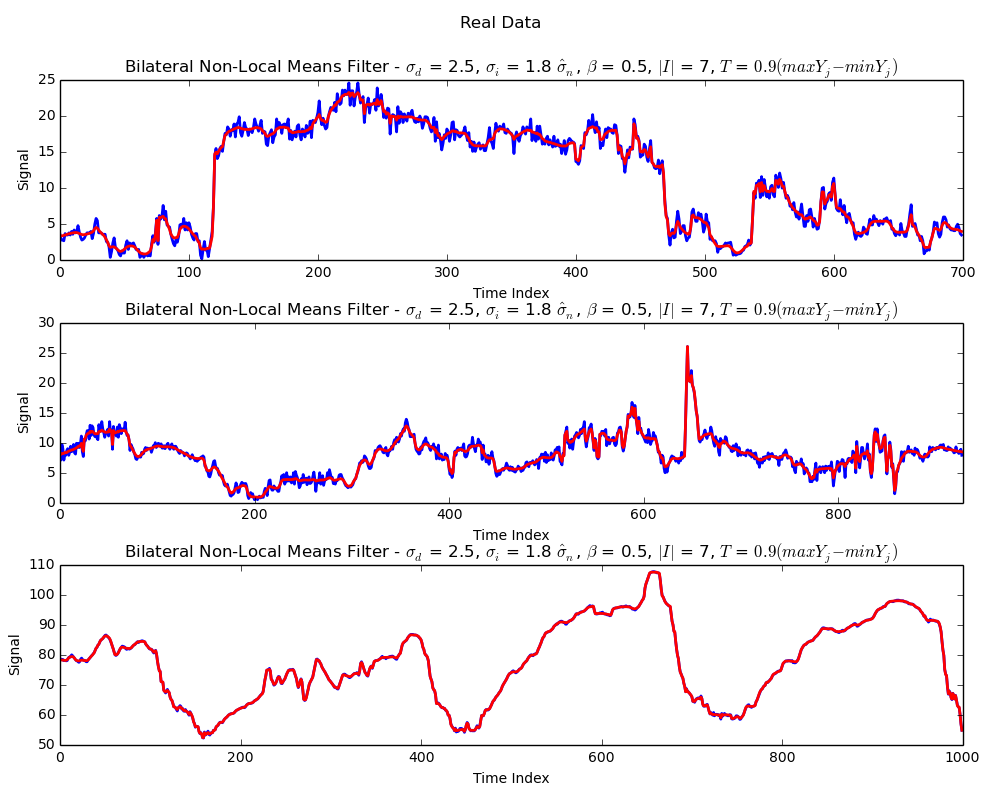
\includegraphics[width = 0.75 \textwidth]{BilateralNLMeansRealCompare.png}

\end{center}
\end{frame}

%------------------------------------------------
\section{Summary}
%------------------------------------------------

\begin{frame}
\begin{center}
\frametitle{Comparison}

\small{

Selected Performance at 10\% Noise

\begin{table}[h]
\begin{tabular}{l | l | l | l}
 & Time Series 1 & Time Series 2 & Time Series 3 \\ \hline
Noisy &62.771 &60.905 & 66.585 \\ \hline
Box Filter &73.249/98.9\% &66.040/99.8\% & 64.923/99.3\% \\ \hline
Gaussian Filter & 75.844/100.0\% & 67.568/98.4\% & 62.980/91.0\% \\ \hline
\cellcolor{airforceblue}Bilateral Filter & \cellcolor{aliceblue}79.580/97.3\% & 75.578/96.7\% & \cellcolor{aliceblue}84.480/99.4\% \\ \hline
Non-Local Means & 77.760/95.7\% & 75.828/95.1\% & 79.996/98.8\% \\ \hline
\cellcolor{airforceblue}Bilateral NL-Means & \cellcolor{aliceblue}79.659/91.4\% & \cellcolor{aliceblue}78.388/94.9\% & 77.953/89.7\%
\end{tabular}
\end{table}

}

\end{center}
\end{frame}

%------------------------------------------------

\begin{frame}
\begin{center}
\frametitle{Summary}

The Bilateral and Bilateral/Non-Local Means filters do a good job smoothing and appear to have stable optimal parameters

\end{center}
\end{frame}

%------------------------------------------------

\begin{frame}
\begin{center}
\frametitle{Acknowledgements}

Collaborators:

\begin{itemize}

\item Dr Ya Ju Fan

\item Dr Chandrika Kamath

\end{itemize}

$ $\\

SensorStreams project funded by ASCR Applied Math Program\\

$ $\\

LLNL IM Release: LLNL-PRES-657747

\end{center}
\end{frame}

%------------------------------------------------

\begin{frame}
\begin{center}
\frametitle{Future Research}

\begin{enumerate}

\item Different noise models

\item Longer simulated time series

\item Different simulated time series

\item Improved maximum intensity windows difference estimate

\end{enumerate}

\end{center}
\end{frame}

%------------------------------------------------
\section{}
%------------------------------------------------

\begin{frame}
\titlepage % Print the title page
\end{frame}

%------------------------------------------------

\begin{frame}
\begin{center}
\frametitle{Extra Slides}

Extra Slides

\end{center}
\end{frame}

%------------------------------------------------

\begin{frame}
\begin{center}
\frametitle{Frequency Transform Coefficient Hard Thresholding}

$v\left(\alpha\right)$ represents the transformed data, the frequency coefficients

\begin{displaymath}
v\left(\alpha\right) = 
\begin{cases}
v\left(\alpha\right) & \lvert v\left(\alpha\right)\rvert > \mu \\
0 & \lvert v\left(\alpha\right)\rvert < \mu
\end{cases}
\end{displaymath}

$ $\\

$ $\\

Parameter: $\mu$

\end{center}
\end{frame}

%------------------------------------------------

\begin{frame}
\begin{center}
\frametitle{Frequency Transform Coefficient Soft Thresholding}

$v\left(\alpha\right)$ represents the transformed data, the frequency coefficients

\begin{displaymath}
v\left(\alpha\right) = 
\begin{cases}
v\left(\alpha\right) - \mu & \lvert v\left(\alpha\right)\rvert > \mu \\
0 & \lvert v\left(\alpha\right)\rvert < \mu
\end{cases}
\end{displaymath}

$ $\\

$ $\\

Parameter: $\mu$

\end{center}
\end{frame}

%------------------------------------------------

\begin{frame}
\titlepage % Print the title page
\end{frame}

%------------------------------------------------

%----------------------------------------------------------------------------------------

\end{document} 
